\section{Data smashing}
	% Need to change the point of view, I believe
	Data smashing\cite{data_smashing} is a new way to compare data stream from different stochastic sources, and evaluate their similarity (Figure \ref{fig:similar}).
	What we call data stream is for instance a continuous signal, which can be encoded with an alphabet, which will map values to letters (each letter will represent a data range of the values). 
	For instance, one of the signal in Figure \ref{fig:similar} could be encoded with something like \verb|aaaabacabababcbabcbabaaaa|.
	We also assume that the streams can be produced by a probabilistic finite state automata (which we don't know).

	\begin{figure}[h]
		\begin{center}
			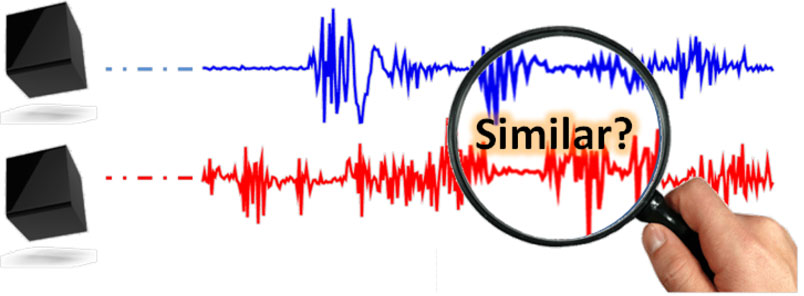
\includegraphics[width=0.8\textwidth]{figures/similar.png}
		\end{center}
		\caption{How to determine if those two streams comes from the same source ?}
		\label{fig:similar}
	\end{figure}

	To do so, we use the concept of anti-stream, which is the "statistical opposite" of a stream: rare letters becomes common in the anti-stream, and common ones become rare. 
	Then, by "smashing" a stream and an anti-stream, we obtain a stream which contain the statistical difference between the two streams, that we now need to process.
	This is done during the last part of the processing, where we calculate the deviation between those two streams.

	Comparing two completely different streams (i.e.: they comes from two different stochastic sources) should produce a high deviation, while comparing streams from the same source (or even comparing a stream against himself) shall yield a deviation close to zero.

	The basic circuit to compare two stream is shown in Figure \ref{fig:circuit}.
	It will produce three deviation values : two of them are the self-annihilation test, to ensure that we have sufficiently long data streams.
	The third is the actual deviation between the two data streams.

	\begin{figure}[h]
		\begin{center}
			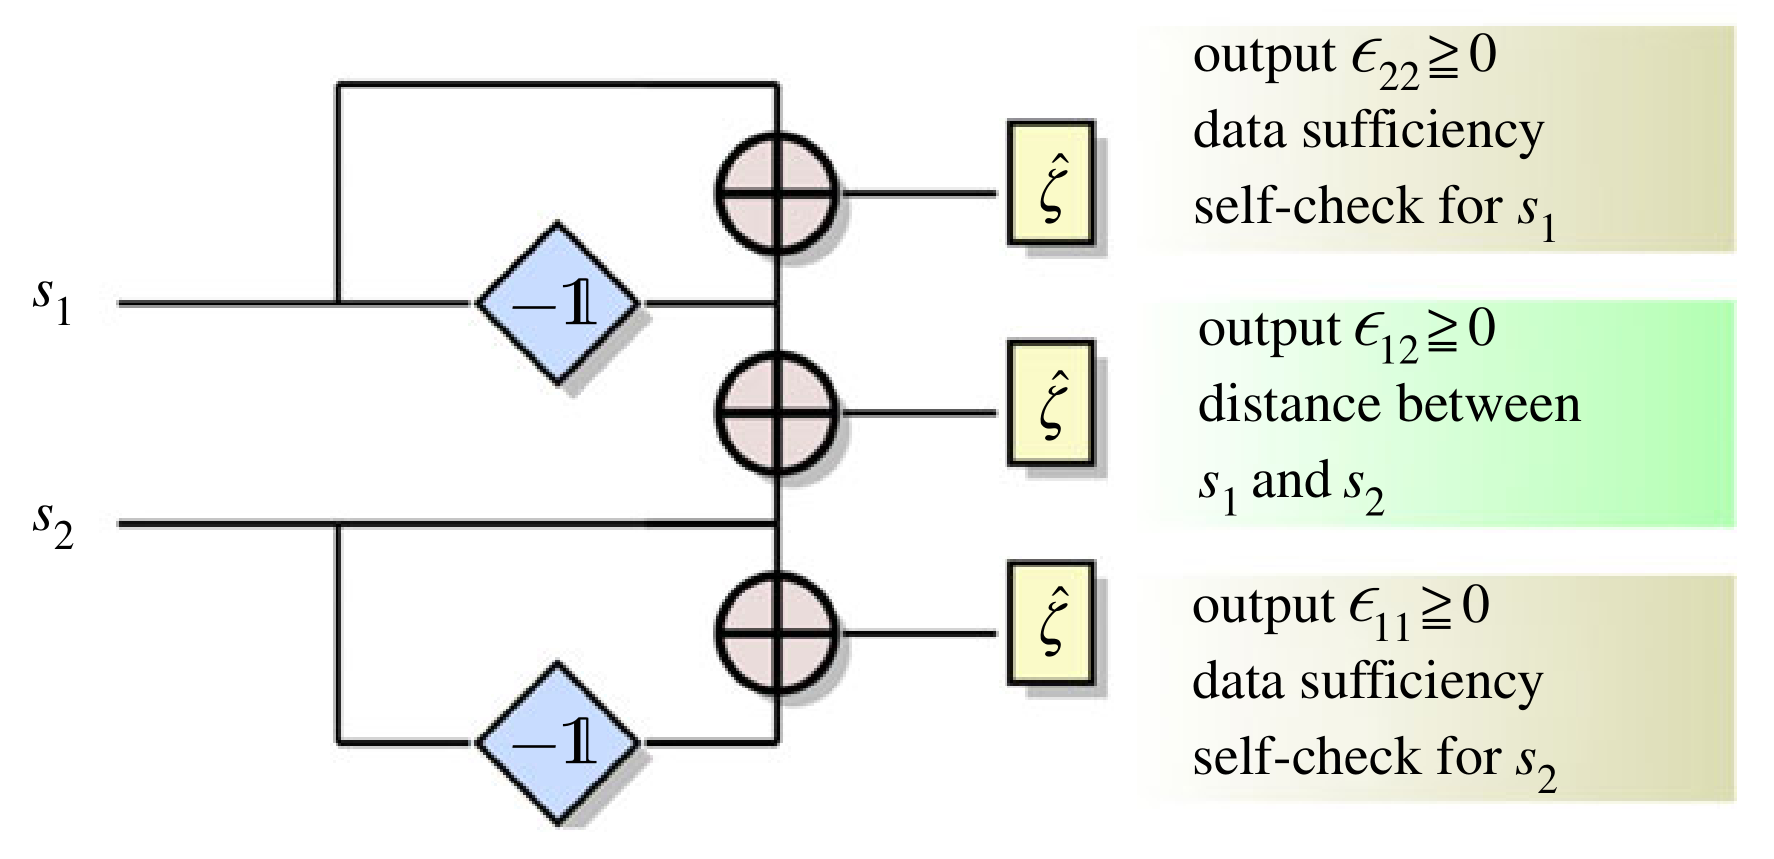
\includegraphics[width=0.8\textwidth]{figures/circuit.png}
		\end{center}
		\caption{This circuit will not only compare the two streams, but also check that the streams are sufficiently long to have meaningful results.}
		\label{fig:circuit}
	\end{figure}

	% Talk about result matrix.

	We will now briefly present the different mechanisms of the algorithm, without going too much into details.
	Detailed explanations about the inner workings of the algorithm can be found in the original paper \cite{data_smashing}.

	\subsection{Stream inversion}
		This process will produce the anti-stream of a stream, which will be collided later to an original stream. 
		The term anti-stream can be counter intuitive. 
		For instance, consider the stream \verb|10111|. Its anti-stream won't be \verb|-10-1-1-1-1|, but a stream that inverted statistical properties of occurrence of the symbols.
		In the end, there may be different anti-stream for a given stream.

		What actually matter, is that the anti-stream could have been produced by a PFSA which is the opposite of the original one (Figure \ref{fig:inversion}).

		\begin{figure}[h]
			\begin{center}
				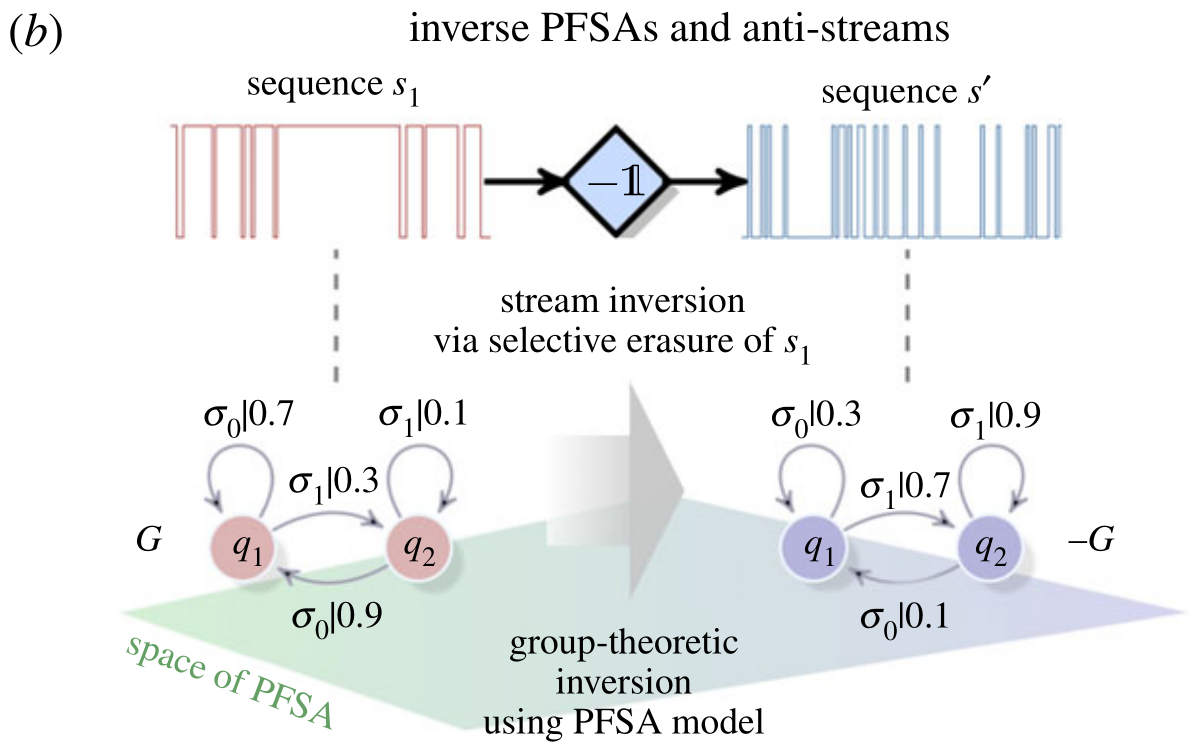
\includegraphics[width=0.8\textwidth]{figures/inversion.png}
			\end{center}
			\caption{The stream inversion will produce a stream similar to a one produced by the opposite PFSA.}
			\label{fig:inversion}
		\end{figure}

	\subsection{Stream summation}
		The second process in the algorithm is the summation (or smashing, colliding) of two streams, and is illustrated in Figure \ref{fig:summation}.

		\begin{figure}[h]
			\begin{center}
				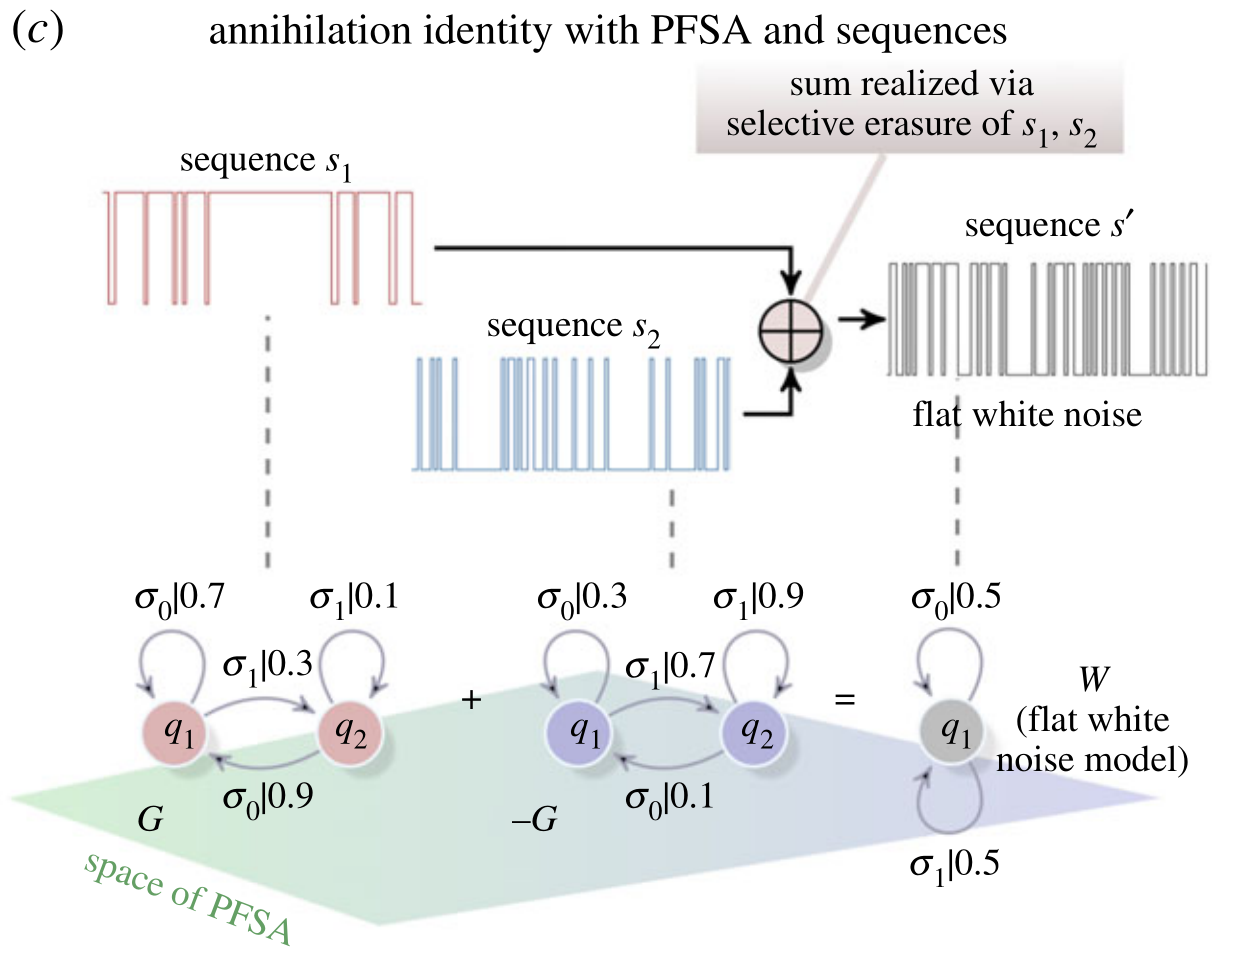
\includegraphics[width=0.8\textwidth]{figures/summation.png}
			\end{center}
			\caption{Summing a stream and its anti-stream will produce flat noise.}
			\label{fig:summation}
		\end{figure}

		Remember that we always sum a stream with an anti-stream, never two streams directly.

	\subsection{Deviation calculation}
		The last part, once we get the smashed stream, it to calculate its deviation from Flat White Noise (FWN).
		The deviation value ($\in [0;1]$) is then compared to a threshold (one input of the algorithm), to determine if the two streams are similar or not.

		INSERT matrix screenshot